\documentclass{article}


\usepackage[T2A]{fontenc}
\usepackage[utf8]{inputenc}
\usepackage[russian]{babel}
\usepackage[pdftex]{graphicx}
\usepackage[unicode, colorlinks, linkcolor=blue]{hyperref}
\graphicspath{{pictures/}}
\DeclareGraphicsExtensions{.pdf,.png,.jpg}


\begin{document}
	\begin{figure}[!]
\centering{
\includegraphics[scale=0.25]{AU}}\\
{\Large\bfseries Санкт-Петербургский национальный исследовательский Академический университет имени Ж.И.~Алфёрова Российской академии наук}
\end{figure}
\begin{center}
Свиридов Фёдор, Александр Слободнюк, Владимир Попов
\end{center}
\rule{12cm}{0.4mm}
\begin{center}
{\large\textbf{Рабочий протокол и отчёт по лабораторной работе № 3}}
\end{center}


\paragraph{Цель работы.}
Вычислить $g$ ускорение свободного падения с помощью математического
и обратного маятника

\paragraph{Задачи, решаемые при выполнении работы.}
\begin{enumerate}
	\item Нахождение центра масс оборотного маятника
	\item Измерение $ T_1 $ периода колебаний оборотного маятника в первой точке подвеса
	\item Измерение $ T_2 $ периода колебаний оборотного маятника во второй точке подвеса
	\item Измерение $ T$ периода колебаний математического маятника
	\item Вычисление $ g $ ускорение свободного падения
	\item Сравнение результатов и подведение выводов
\end{enumerate}

\paragraph{Объект исследования.}
Физическая величина: $ g $  ускорение свободного падения
\paragraph{Метод экспериментального исследования.}

Измерение периода колебаний и расстояния до центра масс




 \paragraph{Рабочие формулы и исходные данные.}\hypertarget{formula}{}
$$g_2=4\pi^2\frac{l}{T^2}\eqno(2)$$
$$g_1=4\pi^2\frac{a_1^2-a_2^2}{T_1^2a_1-T_2^2a_2}\eqno(1)$$
где $ a_1 $ и $ a_2 $ расстояния от центра масс до 1-го и 2-го подвеса, соответственно 
Формула (1) для математического маятника, (2) - для оборотного\\

\begin{table}[h]
	\caption{\bf Измерительные приборы}
\begin{tabular}[c]{|p{7.5em}|p{7.5em}|p{7.5em}| p{7.5em}|}
	\hline
Наименование & Тип прибора & Используемый диапазон & Погрешность прибора\\\hline
Модуль измерительный& Цифровой&$0{,}5 - 1{,}5$ c.&$ 0{,}005 $ c.\\
\hline
	\end{tabular}
\end{table}


\begin{figure}[h]
	\caption{Оборотный маятник}
\centering{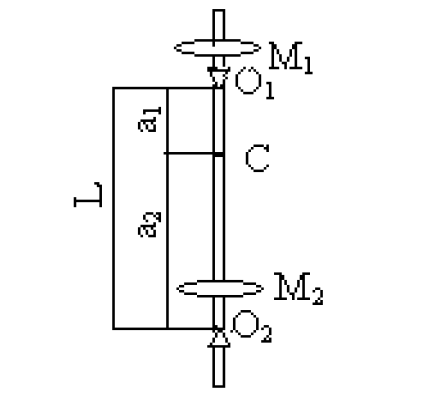
\includegraphics[scale=0.4]{q}}
\end{figure}

\begin{figure}[h]
	\caption{Схема установки}
	\centering{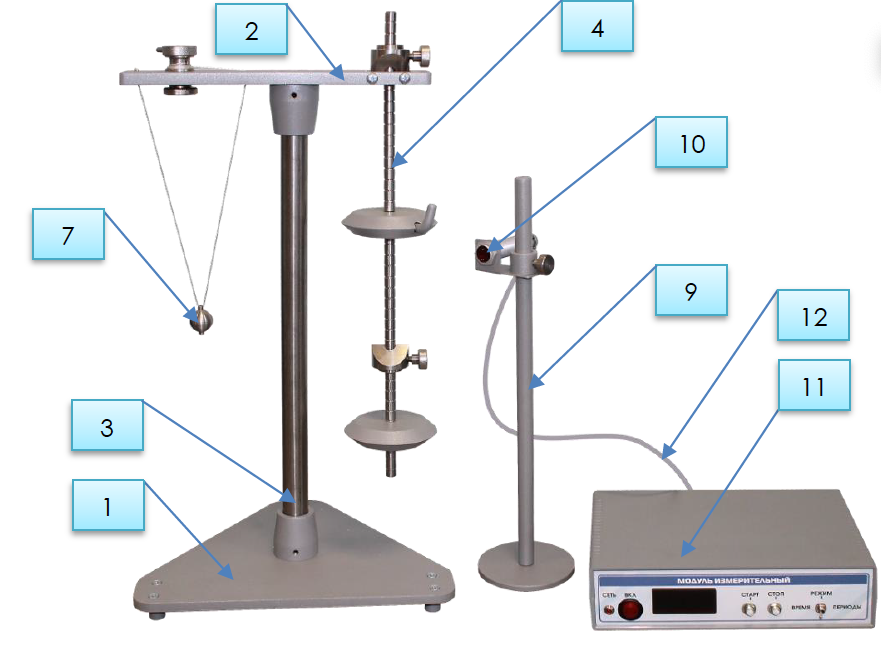
\includegraphics[scale=0.15]{w}}
\end{figure}



\paragraph{Результаты прямых измерений и их обработки }
\begin{enumerate}
	\item Центр масс\\
	$ a_1 = 8 $ см.\\
	$ a_2 = 14$ см.
	
\item Оборотный маятник в первой точке подвеса\\
\begin{table}[!h]	
\begin{tabular}{|c|c|c|}
	\hline
	№ & Число колебаний N & $t_1$  время N колебаний (c.) \\
	\hline
	1 & 5 & 5,355 \\
	\hline
	2 & 5 & 5,357 \\
	\hline
	3 & 5 & 5,359 \\
	\hline
\end{tabular}
\end{table}

\item Оборотный маятник во второй точке подвеса

\begin{table}[!h]
\begin{tabular}{|c|c|c|}
		\hline
		№ & Число колебания N & $t_2$  время N колебаний (c.) \\
		\hline
		1 & 10 & 10,110 \\
		\hline
		2 & 10 & 10,105 \\
		\hline
		3 & 10 & 10,115 \\
		\hline
\end{tabular}
\end{table}

\item Математический маятник

\begin{table}[!hpb]
	\begin{tabular}{|c|c|c|}
		\hline
		№ & Число колебания N & $t$  время N колебаний (c.) \\
		\hline
		1 & 10 &  9,901\\
		\hline
		2 & 10 & 9,921 \\
		\hline
		3 & 10 & 9,918 \\
		\hline
	\end{tabular}
\end{table}
\end{enumerate}

\paragraph{Расчет результатов косвенных измерений }
\begin{enumerate}
\item Период колебания оборотного маятника в первой точке подвеса
$$T_1\approx\frac{<t_1>}{N}\approx 1{,}0714\quad(\mbox{c}) $$
\item Период колебания оборотного маятника во второй точке подвеса
$$T_2\approx\frac{<t_2>}{N}\approx 1{,}0110\quad(\mbox{c})  $$
\item Период колебания математического маятника
$$T\approx\frac{<t>}{N}\approx 0{,}9913\quad(\mbox{c})  $$
\item Ускорение свободного падения $g_1$\\
\hyperlink{formula}{По формуле (1):}

$$ g_1 = 4\pi^2\,\frac{0,08^2-0,14^2}{0,08\cdot1,071^2-0,14\cdot1,011^2}\approx10,2 \quad\left(\frac{\mbox{м}}{\mbox{с}^2}\right)$$
\begin{center}
	\fbox{$ g_1\approx 10,2\quad\left(\frac{\mbox{м}}{\mbox{с}^2}\right) $}
\end{center}

\item Ускорение свободного падения $g_2$\\
\hyperlink{formula}{По формуле (2):}

$$ g_2=4\pi^2\,\frac{0,22}{0,9913^2}\approx8,8\quad\left(\frac{\mbox{м}}{\mbox{с}^2}\right)$$
\begin{center}
	\fbox{$g_2\approx 8,8\quad\left(\frac{\mbox{м}}{\mbox{с}^2}\right)$}
\end{center}



\end{enumerate}

\paragraph{Расчет погрешностей измерений }
\begin{enumerate}
	\item Для оборотного маятника\\
	$\Delta L_1 =2\cdot10^{-3} \quad(\mbox{м})$\\
	$L_1 = 22 \quad(\mbox{см})$\\
	$\Delta t_1 = 0,005 \quad(\mbox{c})$\\
	$ <T_1>= 1,041 \quad(\mbox{c})$
	$$\frac{\Delta g_1}{g_1}\approx\sqrt{\left(\frac{\Delta L_1}{L_1}\right)^2+4\left(\frac{\Delta t_1}{<T_1>}\right)^2}\approx0,013$$
	$$ \Delta g_1\approx0,1\quad\left(\frac{\mbox{м}}{\mbox{с}^2}\right)$$
		\item Для математического маятника\\
	$\Delta L_2 =5\cdot10^{-3} \quad(\mbox{м})$\\
	$L_2 = 22 \quad(\mbox{см})$\\
	$\Delta t_2 = 0,005 \quad(\mbox{c})$\\
	$ <T_2>= 0,9913 \quad(\mbox{c})$
	$$\frac{\Delta g_2}{g_2}\approx\sqrt{\left(\frac{\Delta L_2}{L_2}\right)^2+4\left(\frac{\Delta t_2}{<T_2>}\right)^2}\approx0,025$$
	$$ \Delta g_1\approx0,2 \quad\left(\frac{\mbox{м}}{\mbox{с}^2}\right)$$
\end{enumerate}

\paragraph{Окончательные результаты.}
$$ g_1=(10,2\pm0,1)\quad\frac{\mbox{м}}{\mbox{с}^2}$$
$$ g_2=(8,8\pm0,2)\quad\frac{\mbox{м}}{\mbox{с}^2}$$

\paragraph{Выводы и анализ результатов}
Мы вычислили ускорение свободного падения с помощью двух маятников: математического и оборотного. Полученные результаты довольно сильно отличаются, данную ситуацию можно объяснить тем, что, несмотря на довольно точное измерение периода, в первом случае были трудности с измерением центра масс, а во втором - с измерением длины маятника.
\end{document}
